
\caulc
\Opensolutionfile{ans}[ans/ansTN-Dung]
%%=============EX_1=============%%%
\begin{ex}%[2D1N4-1]%[TDMT08]%[Bồ Văn Hậu]
	\immini[thm]{Cho hàm số $y=\dfrac{ax+b}{cx+d}$, với $c\ne 0$ và $ad\ne bc$ có đồ thị như hình vẽ bên. Hỏi tiệm cận đứng của đồ thị hàm số trên là đường thẳng nào?
		\choice
		{$y=1$}
		{$x=2$}
		{$y=2$}
		{\True $x=1$}}{
		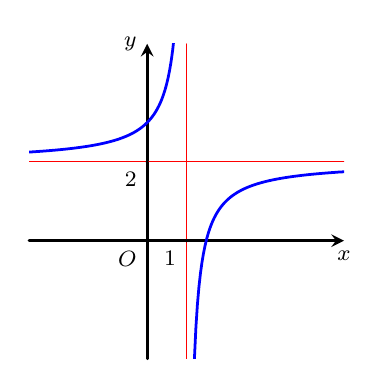
\begin{tikzpicture}[declare function={a=-3; b=5; c=-3; d=5;}, scale=0.5, font=\footnotesize, line join=round, line cap=round, >=stealth, line width=1pt]
			\draw[->] (a,0)--(b,0) node[below]{$x$};
			\draw[->] (0,c)--(0,d) node[left]{$y$};
			\clip (a,c) rectangle (b,d);
			\draw[samples=100,blue] plot[domain=a:0.8] ({\x},{(2*\x-3)/(\x-1)});
			\draw[samples=100,blue] plot[domain=1.2:b] ({\x},{(2*\x-3)/(\x-1)});
			\draw[thin,red] (a,2)--(b,2) (1,c)--(1,d);
			\fill (0,0) circle(1.2pt) node[below left]{$O$} 
			(1,0) circle(1.2pt) node[below left]{$1$} 
			(0,2) circle(1.2pt) node[below left]{$2$};
	\end{tikzpicture}}
	\loigiai{
		Dựa vào đồ thị ta thấy tiệm cận đứng của đồ thị hàm số là đường thẳng $x=1$.
	}
\end{ex}
%%%=============================%%%

%%%=============EX_2=============%%%
\begin{ex}%[1D6H4-3]%[TDMT08]%[Đình Nguyên]
	Tập nghiệm của bất phương trình $\log_{\frac{1}{3}}(x-2) > -2$ là
	\choice
	{\True $(2;11)$}
	{$(2;9)$}
	{$(9;+\infty)$}
	{$(-\infty;11)$}
	\loigiai{
		Điều kiện xác định $x - 2 > 0 \Leftrightarrow x > 2$.\\
		Bất phương trình tương đương với
		$x - 2 < \left( \dfrac{1}{3} \right)^{-2} \Leftrightarrow x - 2 < 9 \Leftrightarrow x < 11$.\\
		Kết hợp điều kiện, ta được tập nghiệm là $(2;11)$.
	}
\end{ex}
%%%=============================%%%

%%%=============EX_3=============%%%
\begin{ex}%[2H2N2-3]%[TDMT08]%[Trần Văn Thiện]
	Trong không gian $Oxyz$, cho hai vectơ $\overrightarrow{u}=(1;2;0)$ và $\overrightarrow{v}=(-2;1;-1)$. Tổng của hai vectơ này có tọa độ là
	\choice
	{$(3;1;1)$}
	{\True $(-1;3;-1)$}
	{ $(-3;-1;-1)$}
	{$(1;-2;1)$}
	\loigiai{ 
		Vì $\overrightarrow{u}=(1;2;0)$ và $\overrightarrow{v}=(-2;1;-1)$ nên $\overrightarrow{u}+\overrightarrow{v}=(1-2;2+1;0-1)=(-1;3;-1)$. 
	}
\end{ex}
%%%=============================%%%

%%%=============EX_4=============%%%
\begin{ex}%[2D1N1-2]%[TDMT08]%[Mui Doan]
	\immini[thm]{
		Cho đồ thị của hàm số $y=f(x)$ như hình vẽ bên. Hỏi hàm số $f(x)$ nghịch biến trên khoảng nào dưới đây?
		\choice
		{$(-5;+\infty)$}
		{\True $(-1;4)$}
		{$(4;+\infty)$}
		{$(-\infty;4)$}}
	{
		\begin{tikzpicture}[declare function={xmin=-6; xmax=6.5; ymin=-1; ymax=5; f(\x)=0.01*(\x)^3-0.18*(\x)^2-0.38*(\x)+3.81; g(\x)=0.09*(\x)^3-0.46*(\x)^2-0.55*(\x)+3.82;}, line cap=butt, line join=miter, >=stealth, xscale=0.7]
			\draw[->] (xmin,0)--(xmax,0) node[shift={(-100:7pt)},font=\normalsize]{$x$};
			\draw[->] (0,ymin)--(0,ymax) node[shift={(190:7pt)},font=\normalsize]{$y$};
			\fill (0,0) node[shift={(130:9pt)},font=\normalsize]{$O$};
			\filldraw (-5,0) circle(1pt) (-1,4) circle(1pt) (4,0) circle(1pt);
			\draw[dashed] (-5,0) node[above left]{$-5$} (-1,0) node[below]{$-1$} -- (-1,4) (4,0) node[below]{$4$};
			\node[left] at (6,4) {$f(x)$};
			\clip (xmin,ymin) rectangle (xmax,ymax);
			\draw[smooth, samples=150, domain=xmin:0] plot (\x, {f(\x)});
			\draw[smooth, samples=150, domain=0:xmax] plot (\x, {g(\x)});
		\end{tikzpicture}
	}
	\loigiai{
		Theo đồ thị, ta có hàm số nghịch biến trên $(-1;4)$.
	}
\end{ex}
%%%=============================%%%

%%%=============EX_5=============%%%
\begin{ex}%[2D1H2-1]%[TDMT08]%[Nguyễn Trí Minh Tuấn]
	Cực tiểu của hàm số $y=x^3-3x$ là
	\choice
	{$(1;-2)$}
	{$(-1;2)$}
	{$x=1$}
	{\True $y=-2$}
	\loigiai{
		Ta có $y'=3x^2-3=0 \Leftrightarrow 3x^2-3=0 \Leftrightarrow x=\pm1$.\\
		Lại có $y''=6x$, khi đó $y''(1)=6>0$.\\
		Suy ra $x=1$ là điểm cực tiểu.\\
		Vậy, cực tiểu của hàm số là $y(1)=1-3=-2$.
	}
\end{ex}
%%%=============================%%%

%%%=============EX_6=============%%%
\begin{ex}%[TDMT8]%[2H2N2-2]%[Huỳnh Quốc Đạt]
	Trong không gian $Oxyz$, cho điểm $A(2;3;-1)$. Toạ độ điểm đối xứng với $A$ qua mặt phẳng $(Oxy)$ là
	\choice
	{$(2;3;0)$}
	{\True $(2;3;1)$}
	{$(-2;-3;-1)$}
	{$(2;3;-1)$}
	\loigiai{ Toạ độ điểm đối xứng với $A(2;3;-1)$ qua mặt phẳng $(Oxy)$ là $(2;3;1)$.}
\end{ex}
%%%=============================%%%

%%%=============EX_7=============%%%
\begin{ex}%[2D1H2-2]%[TDMT08]%[Chu Ha]
	\immini[thm]{
		Cho đồ thị hàm số $y=f'(x)$ như hình vẽ. Hỏi hàm số $f(x)$ có tất cả bao nhiêu điểm cực đại?
		\choice
		{$4$}
		{$1$}
		{$3$}
		{\True $2$}
	}{
		\begin{tikzpicture}[>=stealth, scale=0.5, line join=round, line cap=round]
			\draw[->] (-4,0) -- (5,0) node[right] {$x$};
			\draw[->] (0,-2.5) -- (0,4) node[above] {$y$};
			\node[below left] at (0,0) {$O$};
			\draw (-4,3)..controls +(280:5) and +(260:5)..(-1,1)..controls +(80:4) and +(250:6)..(2,2)..controls +(68:3) and +(95:3)..(4,-2);
			\foreach \x/\y in {-2.2/-1.8, -0.63/2.1, 0/0, 0.7/0, 2.75/3} {
				\filldraw[blue] (\x,\y) circle (2pt);
			}
			\node[right] at (3,3) {$f'(x)$};
		\end{tikzpicture}
	}
	\loigiai{
		Ta có các điểm cực đại của hàm số $f(x)$ tương ứng với các điểm mà tại đó $f'(x)$ đổi dấu từ dương sang âm.\\
		Trên đồ thị $f'(x)$ có đúng $2$ điểm đổi dấu từ $+$ sang $-$.\\
		Suy ra hàm số $f(x)$ có tất cả $2$ điểm cực đại.
	}
\end{ex}
%%%=============================%%%

%%%=============EX_8=============%%%
\begin{ex}%[2H2N2-4]%[TDMT08]%[Nguyễn Tấn Linh]
	Trong không gian $Oxyz$, cho vectơ $\overrightarrow{u}=(1;2;-3)$ và điểm $A(3;0;-2)$. Tích vô hướng của hai vectơ $\overrightarrow{u}$ và $\overrightarrow{AO}$ bằng
	\choice
	{\True $-9$}
	{$9$}
	{$6$}
	{$7$}
	\loigiai{
		Ta có $O(0;0;0)$ là gốc tọa độ, suy ra $\overrightarrow{AO}=(-3;0;2)$.\\
		Khi đó tích vô hướng
		\[ \overrightarrow{u}\cdot\overrightarrow{AO}=1\cdot(-3)+2\cdot 0+(-3)\cdot 2=-3+0-6=-9. \]
	}
\end{ex}
%%%=============================%%%

%%%=============EX_9=============%%%
\begin{ex}%[1H8H4-2]%[TDMT08]%[Lê Phúc]
	Cho hình chóp $S.ABCD$ có đáy $ABCD$ là hình vuông, có $SA\perp (ABCD)$. Trong các mặt phẳng dưới đây, mặt phẳng \textbf{không} vuông góc với mặt phẳng $(SAC)$ là
	\choice
	{$(ABCD)$}
	{$(SBD)$}
	{\True $(SCD)$}
	{$(BCD)$}
	\loigiai{
		\immini{
			\begin{itemize}
				\item Ta có $\heva{&SA\perp (ABCD)\\&SA\subset (SAC)}\Rightarrow (SAC)\perp (ABCD)$.
				\item Ta có $\heva{&SA\perp (BCD)\\&SA\subset (SAC)}\Rightarrow (SAC)\perp (BCD)$.
				\item Ta có $\heva{&BD\perp SA\\&BD\perp AC}\Rightarrow BD\perp (SAC)$.\\
				Mặt khác $BD\subset(SBD)$ nên $(SAC)\perp (SBD)$.
			\end{itemize}
			Vậy $(SCD)$ không vuông góc với $(SAC)$.
		}{
			\begin{tikzpicture}[declare function={a=3; b=2; h=2.5;}, line join=round, line cap=round, >=stealth]
				\path 
				(0,0) coordinate (A)
				(a,0) coordinate (D)
				(-135:b) coordinate (B)
				($(B)+(D)$) coordinate (C)
				(0,h) coordinate (S);
				
				\path pic[draw,angle radius=5pt]{right angle=B--A--S};
				\path pic[draw,angle radius=5pt]{right angle=D--A--S};
				
				\draw[dashed] (B)--(A)--(D) (A)--(S);
				\draw (S)--(B)--(C)--(D)--cycle (S)--(C);
				
				\foreach \t/\g in {A/180, B/180, C/0, D/0, S/90} {
					\filldraw (\t) circle (1pt) node[shift={(\g:9pt)},font=\scriptsize]{$\t$};
				}
		\end{tikzpicture}}
	}
\end{ex}
%%%=============================%%%

%%%=============EX_10=============%%%
\begin{ex}%[1D7N2-1]%[TDMTD08]%[Phạm Hải Dương]
	Biểu thức đạo hàm của hàm số $y=\mathrm{e}^x$ là
	\choice
	{$y'=x\mathrm{e}^{x-1}$}
	{$y'=\dfrac{\mathrm{e}^{x+1}}{x+1}$}
	{$y'=3^x \ln 3$}
	{\True $y'=\mathrm{e}^x$}
	\loigiai{
		Theo bảng công thức đạo hàm của các hàm số sơ cấp cơ bản, ta có $\left(\mathrm{e}^x\right)' = \mathrm{e}^x$.
	}
\end{ex}
%%%=============================%%%

%%%=============EX_11=============%%%
\begin{ex}%[1D2N3-3]%[TDMTD08]%[Trí Thiện]
	Cho cấp số nhân $(u_n)$ có $u_1 = 2$ và công bội $q = 1$. Số hạng $u_3$ bằng
	\choice
	{$4$}
	{$8$}
	{\True $2$}
	{$3$}
	\loigiai{
		Ta có công thức số hạng tổng quát của cấp số nhân là $u_n = u_1 \cdot q^{n-1}$.\\
		Khi đó số hạng $u_3$ là
		\[u_3 = u_1 \cdot q^{3-1} = 2 \cdot 1^2 = 2.\]
	}
\end{ex}
%%%=============================%%%

%%%=============EX_12=============%%%
\begin{ex}%[2H2H1-2]%[TDMT08]%[Nguyễn Sơn Thành]
	Cho hình hộp $ABCD.A'B'C'D'$. Hỏi phát biểu nào sau đây đúng?
	\immini{
		\choice
		{\True $\overrightarrow{AB} + \overrightarrow{B'C'} + \overrightarrow{DD'} = \overrightarrow{AC'}$}
		{$\overrightarrow{AB} + \overrightarrow{AD'} + \overrightarrow{CC'} = \overrightarrow{AC'}$}
		{$\overrightarrow{AB} + \overrightarrow{BC} + \overrightarrow{BC'} = \overrightarrow{AC'}$}
		{$\overrightarrow{AA'} + \overrightarrow{BB'} + \overrightarrow{CC'} = \overrightarrow{AC'}$}
	}{
		\begin{tikzpicture}[line cap=round, line join=round, font=\footnotesize, >=stealth, scale=0.7]
			\path 
			(0,0) coordinate (A)
			(5,0) coordinate (D)
			(-2,-2) coordinate (B)
			($(D) - (A) + (B)$) coordinate (C)
			($(A) + (0.5,3)$) coordinate (A')
			($(B) + (0.5,3)$) coordinate (B')
			($(C) + (0.5,3)$) coordinate (C')
			($(D) + (0.5,3)$) coordinate (D');
			
			\draw[dashed] (A')--(A)--(C') (B)--(A)--(D);
			\draw (A')--(B')--(C')--(D')--cycle (D')--(D)--(C) (B')--(B)--(C)--(C')--cycle;
			
			\foreach \i/\r in {A/180, B/-135, C/-45, D/0, A'/105, B'/180, C'/-45, D'/45} {
				\filldraw[black] (\i) circle (1pt);
				\node at ($(\i) + (\r:4mm)$) {$\i$};
			}
		\end{tikzpicture}
	}
	\loigiai{
		Ta có $\overrightarrow{AC'} = \overrightarrow{AB} + \overrightarrow{AD} + \overrightarrow{AA'} = \overrightarrow{AB} + \overrightarrow{B'C'} + \overrightarrow{DD'}$.
	}
\end{ex}
%%%=============================%%%
\Closesolutionfile{ans}

\cauds
\Opensolutionfile{ans}[ans/ansTN-DungSai]
%%%=============EX_13=============%%%
\begin{ex}%[2H2H2-5]
	Trong không gian $Oxyz$, cho ba điểm $A(1;2;-1)$, $B(2;4;1)$, $C(3;0;0)$.
	\choiceTF[t]
	{\True $\overrightarrow{AB} = (1;2;2)$}
	{\True Tam giác $ABC$ cân tại $A$}
	{Bán kính đường tròn ngoại tiếp của tam giác $ABC$ bằng $\sqrt{3}$}
	{Bán kính đường tròn nội tiếp của tam giác $ABC$ bằng $3 - \sqrt{2}$}
	\loigiai{
		Ta có $\overrightarrow{AB} = (1;2;2)$, $\overrightarrow{AC} = (2;-2;1)$ và $\overrightarrow{BC} = (1;-4;-1)$.\\
		Suy ra $AB = \sqrt{1^2 + 2^2 + 2^2} = 3$, $AC = \sqrt{4 + 4 + 1} = 3$, $BC = \sqrt{1 + 16 + 1} = 3\sqrt{2}$.
		\begin{itemchoice}
			\itemch $\overrightarrow{AB} = (2-1; 4-2; 1-(-1)) = (1;2;2)$.
			\itemch Vì $AB = AC = 3$ nên tam giác $ABC$ cân tại $A$.
			\itemch Tính diện tích tam giác $ABC$, ta có
			\[\left[\overrightarrow{AB}, \overrightarrow{AC}\right] = \left( 
			\begin{vmatrix} 2 & 2 \\ -2 & 1 \end{vmatrix}; 
			\begin{vmatrix} 2 & 1 \\ 1 & 2 \end{vmatrix}; 
			\begin{vmatrix} 1 & 2 \\ 2 & -2 \end{vmatrix} \right) = (6; 3; -6).\]
			$\left|\left[\overrightarrow{AB}, \overrightarrow{AC}\right]\right| = \sqrt{36 + 9 + 36} = 9$.\\
			Diện tích $S = \dfrac{1}{2} \cdot 9 = \dfrac{9}{2}$.\\
			Bán kính ngoại tiếp $R = \dfrac{AB \cdot BC \cdot CA}{4S} = \dfrac{3 \cdot 3\sqrt{2} \cdot 3}{4 \cdot \dfrac{9}{2}} = \dfrac{3\sqrt{2}}{2} \neq \sqrt{3}$.
			\itemch Nửa chu vi $p = \dfrac{AB + BC + CA}{2} = \dfrac{3 + 3\sqrt{2} + 3}{2} = \dfrac{6 + 3\sqrt{2}}{2}$.\\
			Bán kính nội tiếp $r = \dfrac{S}{p} = \dfrac{\dfrac{9}{2}}{\dfrac{6 + 3\sqrt{2}}{2}} = \dfrac{3\left(2-\sqrt{2}\right)}{2} \neq 3 - \sqrt{2}$.
		\end{itemchoice}
	}
\end{ex}
%%%=============================%%%

%%%=============EX_14=============%%%
\begin{ex}%[2D1V2-1]%[TDMT08]%[Vũ Hồng Toàn]
	Cho hàm số $y = f(x) = x^4 - 2x^2 - 3$ có đồ thị $(C)$.
	\choiceTF[t]
	{\True Đồ thị $(C)$ có ba điểm cực trị}
	{\True $f(x)$ đồng biến trên các khoảng $(-1;0)$ và $(1;+\infty)$}
	{Các điểm cực trị của $(C)$ tạo thành một đa giác có diện tích bằng $2$}
	{\True Trên mặt phẳng tọa độ có hai điểm phân biệt tạo với ba điểm cực trị của $(C)$ thành một hình bình hành (không phải là hình thoi). Hai điểm này cách nhau một đoạn bằng $4$}
	\loigiai{
		Ta có $f(x) = x^4-2x^2-3\Rightarrow f'(x) = 4x^3-4x$.\\
		Cho $f'(x) = 0 \Leftrightarrow 4x^3-4x = 0 \Leftrightarrow \hoac{&x=0\\&x=-1\\&x=1.}$\\
		Bảng biến thiên
		\begin{center}
			
\begin{tikzpicture}
				\tkzTabInit[lgt=1.2, espcl=2.5, deltacl=0.5]
				{$x$/0.7, $f'(x)$/0.7, $f(x)$/2}
				{$-\infty$,$-1$,$0$,$1$,$+\infty$}
				\tkzTabLine{,-,0,+,0,-,0,+}
				\tkzTabVar{+/$+\infty$,-/$-4$,+/$-3$,-/$-4$,+/$+\infty$}
			\end{tikzpicture}
		\end{center}
		Quan sát bảng biến thiên ta nhận thấy
		\begin{itemchoice}
			\itemch Hàm số đã cho có $3$ điểm cực trị (hai cực tiểu tại $x = \pm 1$ và một cực đại tại $x = 0$).
			\itemch Hàm số đã cho đồng biến trên các khoảng $(-1;0)$ và $(1;+\infty)$.
			\itemch Các điểm cực trị của đồ thị $(C)$ là $A(0; -3)$, $B(1; -4)$, $C(-1; -4)$.
			\begin{center}
				\begin{tikzpicture}[scale=1.2, font=\footnotesize, line join=round, line cap=round, >=stealth]
					\coordinate (O) at (0,0);
					\coordinate (A) at (0,-3);
					\coordinate (B) at (1,-4);
					\coordinate (C) at (-1,-4);
					\coordinate (H) at (0,-4);
					
					\draw[->] (-2,0)--(2,0) node[below]{$x$};
					\draw[->] (0,-5)--(0,1) node[left]{$y$};
					\filldraw (O) circle (1.5pt) node[above right]{$O$};
					
					\draw (A)--(B)--(C)--cycle;
					\draw (A)--(H);
					
					\path pic[draw,angle radius=2mm]{right angle= A--H--C};
					\foreach \x /\gN in {A/135, B/-90, C/-90, H/-45}
					\filldraw (\x) circle (1.5pt) node[shift={(\gN:3mm)}]{$\x$};
				\end{tikzpicture}
			\end{center}
			Gọi $H$ là trung điểm của $BC$. Khi đó $H(0;-4)$, $BC=2$, $AH=1$.\\
			Do đó, diện tích tam giác $ABC$ là $S = \dfrac{1}{2} \cdot BC \cdot AH = \dfrac{1}{2} \cdot 2 \cdot 1 = 1$.
			\itemch Gọi $D$, $M$ và $N$ lần lượt là điểm còn lại của hình bình hành $ABDC$, $ACBM$ và $ABCN$.
			\begin{center}
				\begin{tikzpicture}[scale=1.2, font=\footnotesize, line join=round, line cap=round, >=stealth]
					\coordinate (O) at (0,0);
					\coordinate (A) at (0,-3);
					\coordinate (B) at (1,-4);
					\coordinate (C) at (-1,-4);
					\coordinate (H) at (0,-4);
					\coordinate (D) at (0,-5); 
					\coordinate (M) at (2,-3); 
					\coordinate (N) at (-2,-3);
					
					\draw[->] (-3,0)--(3,0) node[below]{$x$};
					\draw[->] (0,-6)--(0,1) node[left]{$y$};
					\filldraw (O) circle (1.5pt) node[above right]{$O$};
					
					\draw (A)--(B)--(C)--cycle; 
					\draw (B)--(D)--(C);        
					\draw (A)--(H);             
					\draw (M)--(N);             
					\draw (M)--(B);             
					\draw (N)--(C);             
					
					\path pic[draw,angle radius=2mm]{right angle= A--H--C};
					\foreach \x /\gN in {A/135, B/-45, C/-135, H/-45, D/-90, M/90, N/90}
					\filldraw (\x) circle (1.5pt) node[shift={(\gN:3mm)}]{$\x$};
				\end{tikzpicture}
			\end{center}
			Dễ thấy $ABDC$ là hình thoi nên hai hình bình hành thỏa mãn yêu cầu bài toán lần lượt là $ACBM$ và $ABCN$ nên hai điểm cần tìm là $M$ và $N$.\\
			Khi đó $MN=2BC=2\cdot 2=4$.
		\end{itemchoice}
	}
\end{ex}
%%%=============================%%%

%%%=============EX_15=============%%%
\begin{ex}%[2D1H1-5]%[TDMTD08]%[Dương Công Tạo]
	Để loại bỏ $x\%$ chất gây ô nhiễm không khí từ khí thải của một nhà máy, người ta ước tính chi phí cần bỏ ra là $C(x)=\dfrac{400x}{100-x}$ (triệu đồng), với $0\le x < 100$.
	\choiceTF[t]
	{Chi phí cần loại bỏ $30\%$ chất gây ô nhiễm không khí là $172$ triệu đồng \textit{(tính theo triệu đồng và làm tròn kết quả đến hàng phần mười)}}
	{\True Chi phí bình quân để loại bỏ $60\%$ chất gây ô nhiễm không khí là $10$ triệu đồng/$1\%$}
	{\True Không thể loại bỏ hết được ô nhiễm cho dù nhà máy này có bỏ ra rất nhiều chi phí}
	{Chi phí loại bỏ chất gây ô nhiễm không khí của nhà máy ngày một rẻ hơn}
	\loigiai{
		\begin{itemchoice}
			\itemch Chi phí cần loại bỏ $30\%$ chất gây ô nhiễm không khí là 
			\[C(30)=\dfrac{400\cdot 30}{100-30}=\dfrac{12\,000}{70}=\dfrac{1\,200}{7}\approx 171{,}4\text{ (triệu đồng)}.\]
			\itemch Chi phí bình quân để loại bỏ $x\%$ chất gây ô nhiễm không khí là 
			\[ \overline{C(x)}=\dfrac{C(x)}{x}=\dfrac{400}{100-x}.\]
			Do đó, chi phí bình quân để loại bỏ $60\%$ chất gây ô nhiễm không khí là 
			\[\overline{C(60)}=\dfrac{400}{100-60}=10\text{ triệu đồng}/1\%.\]
			\itemch Khi $x\to 100^-$ thì $\lim\limits_{x\to 100^-}{(100-x)}=0$ và $\lim\limits_{x\to 100^-}{400x}=40\,000$. Do đó, $\lim\limits_{x\to 100^-}C(x)=+\infty$.\\
			Điều này có nghĩa là không thể loại bỏ hết được ô nhiễm cho dù nhà máy này có bỏ ra rất nhiều chi phí.
			\itemch Vì $C'(x)=\dfrac{40\,000}{(100-x)^2}>0$, $\forall x\in[0;100)$ nên chi phí loại bỏ chất gây ô nhiễm không khí của nhà máy ngày một đắt hơn.
		\end{itemchoice}
	}
\end{ex}
%%%=============================%%%

%%%=============EX_16=============%%%
\begin{ex}%[2H2V1-4]%[TDMT08]%[Văn Minh Thoại]
	\immini[thm]{
		Một miếng tròn đồng chất được treo song song với mặt phẳng nằm ngang bởi ba sợi dây không dãn xuất phát từ điểm $I$ trên trần nhà lần lượt buộc vào ba điểm $A$, $B$, $C$ trên miếng tròn. Biết độ dài ba đoạn dây đều bằng $x$. Trọng lượng của miếng tròn là $P=240\mathrm{\,N}$, bán kính của miếng tròn (khoảng cách từ tâm $O$ đến các điểm $A$, $B$, $C$) bằng $20\mathrm{\,cm}$. Gọi $F$ là độ lớn của các lực căng $\overrightarrow{F}_1$, $\overrightarrow{F}_2$, $\overrightarrow{F}_3$ trên mỗi sợi dây. Khi đó $F=F(x)$ là một hàm của biến $x$, với $x$ tính bằng centimet và $F(x)$ tính bằng Niutơn.
	}{
		\begin{tikzpicture}[line join=round, line cap=round, >=stealth, scale=1]
			\def\r{3} \def\rb{0.7} \def\h{5}
			\def\gocA{120} \def\gocB{240} \def\gocC{0}
			\coordinate (O) at (0,0);
			\coordinate (I) at (0,\h);
			\coordinate (A) at ({\r*cos(\gocA)},{\rb*sin(\gocA)});
			\coordinate (B) at ({\r*cos(\gocB)},{\rb*sin(\gocB)});
			\coordinate (C) at ({\r*cos(\gocC)},{\rb*sin(\gocC)});
			
			\draw[fill=cyan!30] (O) ellipse ({\r} and {\rb});
			\draw[black] (0,0.2) -- (0.2,0.2) -- (0.2,0);
			\draw[dashed,blue] (I) -- (O);
			\draw[dashed,blue] (O) -- (C) node[midway,below,black] {$20\mathrm{\,cm}$};
			
			\draw[thick,blue] (I) -- (A);
			\draw[->,thick,red] (I) -- ($(I)!0.4!(A)$) node[left,black,xshift=-2pt] {$\overrightarrow{F}_1$};
			\draw[thick,blue] (I) -- (B);
			\draw[->,thick,red] (I) -- ($(I)!0.5!(B)$) node[right,black] {$\overrightarrow{F}_2$};
			\draw[thick,blue] (I) -- (C) node[midway,right,black,xshift=3pt] {$x$};
			\draw[->,thick,red] (I) -- ($(I)!0.4!(C)$) node[above right,black] {$\overrightarrow{F}_3$};
			
			\draw[dashed,red,thick] (O) -- (0,-0.7); 
			\draw[->,red,thick] (0,-0.7) -- (0,-1.5) node[right] {$\overrightarrow{P}$};
			
			\draw (0,\h-0.6) arc (-90:-55:0.6);
			\node at (0.2,\h-0.8) {$\varphi$};
			
			\foreach \x/\g in {I/above, O/above left, A/above left, B/below left, C/right}{
				\filldraw (\x) circle (1pt) node[\g] {$\x$};
			}
			
			% Giá treo cố định
			\draw[ultra thick] (-0.7,\h) -- (0.7,\h);
			\foreach \x in {-0.6,-0.4,-0.2,0,0.2,0.4,0.6}
			\draw (\x,\h) -- (\x+0.1,\h+0.15);
		\end{tikzpicture}
	}
	\choiceTF[t]
	{\True $\overrightarrow{F}_1+\overrightarrow{F}_2+\overrightarrow{F}_3=\overrightarrow{P}$}
	{\True $F(x)=\dfrac{80x}{\sqrt{x^2-400}}$}
	{\True Nếu $x=48\mathrm{\,cm}$ thì $F=80\mathrm{\,(N)}$ \textit{(làm tròn kết quả đến hàng đơn vị)}}
	{\True Biết rằng mỗi sợi dây chỉ chịu tối đa một lực căng bằng $150\mathrm{\,N}$. Khi đó chiều dài tối thiểu của sợi dây là $23{,}6\mathrm{\,cm}$ \textit{(làm tròn đến hàng phần mười)}}
	\loigiai{
		\begin{itemchoice}
			\itemch Theo điều kiện cân bằng lực ta có \[\overrightarrow{F}_1 + \overrightarrow{F}_2 + \overrightarrow{F}_3 + \overrightarrow{P} = \overrightarrow{0}.\]
			\itemch Gọi $\overrightarrow{k}$ là vectơ đơn vị cùng hướng với vectơ $\overrightarrow{OI}$. Do tính đối xứng, góc giữa các sợi dây và trục $OI$ bằng nhau, gọi là $\varphi=\widehat{OIC}$. Ta có
			\allowdisplaybreaks
			\begin{align*}
				\left(\overrightarrow{F}_1 + \overrightarrow{F}_2 + \overrightarrow{F}_3\right) \cdot \overrightarrow{k} &= -\overrightarrow{P} \cdot \overrightarrow{k} \\
				\Leftrightarrow \left|\overrightarrow{F}_1\right| \cos \varphi + \left|\overrightarrow{F}_2\right| \cos \varphi + \left|\overrightarrow{F}_3\right| \cos \varphi &= \left|\overrightarrow{P}\right| \\
				\Leftrightarrow 3F \cos \varphi &= 240\\
				\Rightarrow F \cos \varphi &= 80.
			\end{align*}
			Trong tam giác vuông $IOC$, ta có $\cos\varphi=\dfrac{OI}{IC}=\dfrac{\sqrt{x^2-20^2}}{x}=\dfrac{\sqrt{x^2-400}}{x}$.\\
			Thay vào biểu thức trên ta được $F\cdot\dfrac{\sqrt{x^2-400}}{x}=80\Rightarrow F=\dfrac{80x}{\sqrt{x^2-400}}$.
			\itemch Ta có $F(48)=\dfrac{80\cdot 48}{\sqrt{48^2-400}}=\dfrac{3\,840}{\sqrt{1\,904}}\approx 88\mathrm{\,N}$.
			\itemch Để dây không đứt
			\allowdisplaybreaks
			\begin{align*}
				F(x) &\le 150 \\
				\Leftrightarrow \dfrac{80x}{\sqrt{x^2 - 400}} &\le 150\\
				\Leftrightarrow 8x &\le 15\sqrt{x^2 - 400}.
			\end{align*}
			Bình phương hai vế (với $x>20$), ta được
			\allowdisplaybreaks
			\begin{align*}
				64x^2 &\le 225(x^2 - 400)\\
				\Leftrightarrow 161x^2 &\ge 90\,000\\
				\Leftrightarrow x^2 &\ge \dfrac{90\,000}{161}\\
				\Rightarrow x &\ge 23{,}64.
			\end{align*}
			Vậy chiều dài tối thiểu là $23{,}6\mathrm{\,cm}$.
		\end{itemchoice}
	}
\end{ex}
%%%=============================%%%
\Closesolutionfile{ans}

\caukq 
\Opensolutionfile{ans}[ans/ansTN-DienKhuyet]
%%%=============EX_17=============%%%
\begin{ex}%[TDMT08]%[Lương Pho]%[0D3V2-6]
	\immini[thm]{Từ một đoạn dây thép dài $120\mathrm{\,cm}$ ta uốn thành hình ngũ giác như hình vẽ. Biết góc trên đỉnh bằng $120^\circ$. Hãy xác định giá trị lớn nhất của diện tích hình ngũ giác này theo $\mathrm{cm^2}$ (\textit{làm tròn kết quả đến hàng đơn vị}).
	}{\begin{tikzpicture}[scale=1, font=\footnotesize, line join=round, line cap=round]
			\coordinate (A) at (0,0);
			\coordinate (B) at (4,0);
			\coordinate (C) at (4,1.5);
			\coordinate (D) at (2,2.65);
			\coordinate (E) at (0,1.5);
			
			\draw (A) -- (B) -- (C) -- (D) -- (E) -- cycle;
			\draw[dashed] (E) -- (C);
			\path pic[draw, "$120^\circ$", angle eccentricity=1.5, angle radius=0.4cm] {angle = E--D--C};
	\end{tikzpicture}}
	\par\shortans[0]{965}
	\loigiai{
		Đặt $AB=x>0$, $AE=y>0$. Kẻ đường cao $DH$ của tam giác cân $DEC$.
		\immini{Khi đó $ED=\dfrac{EH}{\sin \widehat{EDH}}=\dfrac{\tfrac{x}{2}}{\sin 60^\circ}=\dfrac{x\sqrt{3}}{3}$.\\
			Chu vi của hình ngũ giác đã cho bằng $120\mathrm{\,cm}$ nên
			\[2y+x+2\cdot \dfrac{x\sqrt{3}}{3}=120\Rightarrow y=60-\dfrac{3+2\sqrt{3}}{6}x.\]
			Diện tích hình ngũ giác là}{
			\begin{tikzpicture}[scale=1, font=\footnotesize, line join=round, line cap=round]
				\coordinate (A) at (0,0);
				\coordinate (B) at (4,0);
				\coordinate (C) at (4,1.5);
				\coordinate (D) at (2,2.65);
				\coordinate (E) at (0,1.5);
				\path 
				($(E)!(D)!(C)$) coordinate (H)
				(A)--(E) node[midway,left] {$y$}
				(A)--(B) node[midway,below] {$x$}
				;			
				\draw (A) -- (B) -- (C) -- (D) -- (E) -- cycle (D)--(H);
				\path pic[draw, angle radius=2mm]{right angle =D--H--E};
				\draw[dashed] (E) -- (C);
				\foreach \x/\g in {A/-90, B/0, C/0, D/90, E/170, H/-90}{
					\filldraw (\x) circle (1pt) node[shift={(\g:7pt)}] {$\x$};
				}
			\end{tikzpicture}
		}
		\allowdisplaybreaks
		\begin{align*}
			S(x) &= S_{ABCE}+S_{\triangle CDE}\\
			&= AB \cdot AE+\dfrac{1}{2}\cdot DE^2\cdot \sin 120^\circ\\
			&= xy+\dfrac{1}{2}\cdot \left(\dfrac{x\sqrt{3}}{3}\right)^2\cdot \sin 120^\circ\\
			&= x\left(60-\dfrac{3+2\sqrt{3}}{6}x\right)+\dfrac{\sqrt{3}x^2}{12}\\
			&= 60x-\dfrac{2+\sqrt{3}}{4}x^2.
		\end{align*}
		Ta thấy $S(x)$ là hàm số bậc hai có hệ số $a<0$ nên hàm số đạt giá trị lớn nhất tại $x=-\dfrac{b}{2a}=\dfrac{120}{2+\sqrt{3}}$ và $\max S(x)=S\left(\dfrac{120}{2+\sqrt{3}}\right)=3\,600\left(2-\sqrt{3}\right)\approx 965\mathrm{\,cm^2}$.
	}
\end{ex}
%%%=============================%%%

%%%=============EX_18=============%%%
\begin{ex}%[2H2V2-5]
	Cho khối chóp cụt đều $ABCD.A'B'C'D'$ có độ dài hai cạnh đáy $AB = 6$, $A'B' = 12$, có chiều cao bằng $8$. Cho hình lập phương $ABCD.MNPQ$ sao cho mặt phẳng $(MNPQ)$ khác phía mặt phẳng $(A'B'C'D')$ so với mặt phẳng $(ABCD)$. Hãy tính khoảng cách giữa hai đường thẳng $MN$ và $DD'$ (\textit{làm tròn kết quả đến hàng phần trăm}).
	\par
	\shortans[0]{3,51}
	\loigiai{
		\immini{Gọi $O$ là tâm của hình vuông $ABCD$.\\
			Chọn hệ trục tọa độ $Oxyz$ như hình vẽ.\\
			Vì $ABCD$ là hình vuông cạnh bằng $6$, ta có tọa độ các đỉnh
			$A(3; -3; 0)$, $B(3; 3; 0)$, $C(-3; 3; 0)$ và $D(-3; -3; 0)$.\\
			Hình lập phương $ABCD.MNPQ$ có cạnh bằng $6$, ta có tọa độ các điểm $M(3; -3; 6)$ và $N(3; 3; 6)$.\\
			Khối chóp cụt đều $ABCD.A'B'C'D'$ có chiều cao $h=8$ và cạnh đáy lớn $A'B'=12$, ta có tọa độ điểm $D'(-6; -6; -8)$.\\
			Ta có các vectơ
			\begin{itemize}
				\item $\overrightarrow{MN} = (0; 6; 0)$.
				\item $\overrightarrow{DD'} = (-3; -3; -8)$.
				\item $\overrightarrow{DM} = (6; 0; 6)$.
			\end{itemize}
		}{
			\begin{tikzpicture}[declare function={a=6; b=2.5; h=5; goc=-135;}, scale=0.8, line join=round, line cap=round, >=stealth, font=\footnotesize]
				\path 
				(0,0) coordinate (D)
				(a,0) coordinate (C)
				(goc:b) coordinate (A)
				($(A)+(a,0)$) coordinate (B)
				($(B)!.5!(D)$) coordinate (O)
				($(O)+(0,h)$) coordinate (S);
				\foreach \x in {A,B,C,D} {
					\path ($(\x)!.5!(S)$) coordinate (\x1);
				}
				\path ($(A1)!.5!(C1)$) coordinate (O1)
				($(A1)!.5!(B1)$) coordinate (M)
				($(B1)!.5!(C1)$) coordinate (N);
				
				\foreach \x in {A1,B1,C1,D1} {
					\path (\x)++(90:h/2) coordinate (\x');
				}
				\draw[dashed] (A)--(D)--(C) (A1)--(D1)--(C1) (D)--(D1)--(D1') (M)--(O1)--(S) (O1)--(N);
				\draw (A)--(B)--(C)--(C1)--(C1')--(D1')--(A1')--(A1)--cycle (B)--(B1)--(C1) (A1)--(B1)--(B1')--(C1') (A1')--(B1');
				\draw[-stealth] (M)--($(O1)!2!(M)$) node[above]{$x$};
				\draw[-stealth] (N)--($(O1)!1.5!(N)$) node[below]{$y$};
				\draw[-stealth] (S)--($(O1)!1.4!(S)$) node[left]{$z$};
				\foreach \x/\goc/\t in {A/-100/A', B/-30/B', C/0/C', O1/-90/O, D/-60/D', A1/150/A, B1/0/B, C1/30/C, D1/150/D, A1'/90/M, B1'/-30/N, C1'/0/P, D1'/90/Q} {
					\filldraw (\x) circle (1pt) node[shift={(\goc:7pt)}]{$\t$};
				}
			\end{tikzpicture}
		}
		\noindent
		Tích có hướng của hai vectơ chỉ phương
		\[\left[\overrightarrow{MN}, \overrightarrow{DD'} \right] = \left( 
		\begin{vmatrix} 6 & 0 \\ -3 & -8 \end{vmatrix}; 
		\begin{vmatrix} 0 & 0 \\ -8 & -3 \end{vmatrix}; 
		\begin{vmatrix} 0 & 6 \\ -3 & -3 \end{vmatrix} \right) = (-48; 0; 18).\]
		Khoảng cách giữa hai đường thẳng $MN$ và $DD'$ là
		\[\mathrm{d}\left(MN, DD'\right) = \dfrac{\left| \left[ \overrightarrow{MN}, \overrightarrow{DD'} \right] \cdot \overrightarrow{DM} \right|}{\left| \left[\overrightarrow{MN}, \overrightarrow{DD'} \right] \right|}= \dfrac{180}{\sqrt{2\,628}} = \dfrac{180}{6\sqrt{73}} = \dfrac{30}{\sqrt{73}} \approx 3{,}51.\]
	}
\end{ex}
%%%=============================%%%

%%%=============EX_19=============%%%
\begin{ex}%[2D1V3-6]%[TDMT08]%[Võ Hiệp]
	Nhà máy X chuyên sản xuất một loại sản phẩm cho nhà máy Y. Hai nhà máy thỏa thuận với nhau rằng: Hàng tháng X cung cấp cho Y tối đa $200$ sản phẩm và tối thiểu $1$ sản phẩm, giá bán mỗi đơn vị sản phẩm là $p(x) = 800 - 0{,}02x^2$ (nghìn đồng), $x$ là số sản phẩm X bán cho Y, hàng tháng X chịu một chi phí cố định để sản xuất loại sản phẩm này là $700$ nghìn đồng và chi phí sản xuất mỗi sản phẩm hết $50$ nghìn đồng. Nếu coi như X chỉ sản xuất theo đơn đặt hàng của Y (tức là tất cả các sản phẩm sản xuất ra, thì Y đều mua hết). Gọi lợi nhuận lớn nhất tính theo nghìn đồng của X trong một tháng sau khi làm tròn đến hàng đơn vị là $L$. Hãy xác định ba chữ số tận cùng của $L$.
	\par
	\shortans[0]{201}
	\loigiai{
		Gọi $x$ là số sản phẩm mà nhà máy X sản xuất và bán cho nhà máy Y. \\
		Theo đề bài, số sản phẩm thỏa mãn điều kiện $1 \le x \le 200$, $x\in\mathbb{N}$.\\
		Giá bán mỗi đơn vị sản phẩm là $p(x) = 800 - 0{,}02x^2$ (nghìn đồng). \\
		Tổng doanh thu $R(x)$ là
		$R(x) = x \cdot p(x) = x(800 - 0{,}02x^2) = 800x - 0{,}02x^3$ (nghìn đồng).\\
		Tổng chi phí $C(x)$ là $C(x) = 700 + 50x$ (nghìn đồng).\\
		Lợi nhuận $P(x)$ là
		\[P(x) = R(x) - C(x) = (800x - 0{,}02x^3) - (700 + 50x)= -0{,}02x^3 + 750x - 700.\]
		Xét hàm số $P(x)$ trên đoạn $[1; 200]$. \\
		Đạo hàm $P'(x) = -0{,}06x^2 + 750$.\\
		Cho $P'(x) = 0\Leftrightarrow -0{,}06x^2 + 750 = 0\Leftrightarrow
		\hoac{&x=50\sqrt{5}\in [1; 200]\\&x=-50\sqrt{5}\notin [1; 200].}$\\
		Giá trị $x = 50\sqrt{5} \approx 111{,}803$. \\
		Vì $x\in\mathbb{N}$. Xét các giá trị nguyên gần $50\sqrt{5}$ trong khoảng $(1; 200)$ là $x=111$ và $x=112$.\\
		Tính giá trị của $P(x)$ tại các điểm $x=1$, $x=111$, $x=112$, $x=200$.\\
		Ta có $P(1)=49{,}98$, $P(111)=55\,197{,}38$, $P(112)=55\,201{,}44$, $ P(200)=-10\,700$.\\
		So sánh các giá trị, ta thấy lợi nhuận lớn nhất là $55\,201{,}44$ khi $x=112$. \\
		Lợi nhuận lớn nhất là 	$L = 55\,201{,}44 \approx 55\,201$ (nghìn đồng).\\
		Vậy ba chữ số tận cùng của $L$ là $201$.
	}
\end{ex}
%%%=============================%%%

%%%=============EX_20=============%%%
\begin{ex}%[2D1V3-6]%[TDMT08]%[Nguyễn Đức Tuấn Anh]
	Người ta muốn truyền tín hiệu từ trạm $A$ đến $B$ nhưng giữa $A$ và $B$ có một bức tường hình hộp chữ nhật rất cao (chắn không cho tín hiệu truyền qua). Người ta sẽ khoét một lỗ nhỏ chỗ tiếp giáp giữa chân tường với mặt đất, xuyên qua vuông góc với bức tường, bắt đầu tại $C$ và ló ra ở $D$ phía bên kia (như hình vẽ). Như vậy, tín hiệu sẽ truyền thẳng từ $A$ đến $C$, rồi từ $C$ đến $D$, rồi từ $D$ thẳng đến $B$. Biết $A$ và $B$ có độ cao so với đất lần lượt bằng $9\mathrm{\,m}$ và $7\mathrm{\,m}$, cách các mặt tường gần nhất lần lượt là $13\mathrm{\,m}$ và $6\mathrm{\,m}$, tường dày $2\mathrm{\,m}$, khoảng cách $AB$ bằng $32\mathrm{\,m}$. Hãy xác định đường đi ngắn nhất của tín hiệu từ $A$ đến $B$ theo đơn vị mét (\textit{làm tròn kết quả đến hàng phần mười}).
	\begin{center}
		\begin{tikzpicture}[declare function={a=5; b=10; goc=-10; g=30; h=4;}, scale=0.9, font=\footnotesize, line join=round, line cap=round, >=stealth]
			\path 
			(0,0) coordinate (M)
			++(90:a) coordinate (N)
			++(goc:b) coordinate (P)
			++(-90:a) coordinate (Q);
			
			\foreach \x in {M,N,P,Q} {
				\path ($(\x)+(g:0.75)$) coordinate (\x');
			}
			\path 
			($(M)!0.275!(Q)$) coordinate (C)
			($(M')!0.275!(Q')$) coordinate (D)
			($(M)!0.15!(Q)$) coordinate (H')
			($(H')+(g-180:3)$) coordinate (H)
			($(H)+(90:3.25)$) coordinate (A)
			($(Q')!0.3!(M')$) coordinate (K')
			($(K')+(g:1.5)$) coordinate (K)
			($(K)+(90:2.5)$) coordinate (B);
			
			\fill[pattern=crosshatch, pattern color=gray!50] (N)--(N')--(P')--(P)--cycle (P)--(Q)--(Q')--(P')--cycle;
			\shade[top color=gray!20, bottom color=gray!60] (M)--(N)--(P)--(Q)--cycle;
			
			\draw (N)--(N')--(P')--(Q')--(Q) (P')--(P) (M)--(N)--(P)--(Q)--cycle ;
			\draw[dashed] (M)--(M')--(N') (M')--(Q') (H')--(H) node[midway,below,sloped]{$13\mathrm{\,m}$}
			(K')--(K) node[midway,below,sloped]{$6\mathrm{\,m}$} 
			(A)--(B) node[midway,above,sloped]{$32\mathrm{\,m}$};
			
			\draw[very thick] (A)--(H) node[midway,left]{$9\mathrm{\,m}$} (B)--(K) node[midway,left]{$7\mathrm{\,m}$};
			\draw[thick,red] (A)--(C);
			\draw[thick,red,dashed] (C)--(D)--(B); 
			
			\filldraw[fill=pink!70] (A) circle (3pt) node[left]{$A$} (B) circle (3pt) node[right]{$B$};
			
			\foreach \t/\gN in {C/-90,D/90,K/-70,H/-90} {
				\filldraw (\t) circle (1.5pt) node[shift={(\gN:7pt)}]{$\t$};
			}
			\draw[<->] ($(Q)+(goc:0.2)$)--($(Q')+(goc:0.2)$) node[sloped,below,midway]{$2\mathrm{\,m}$};
		\end{tikzpicture}
	\end{center}
	\par\shortans[0]{36{,}7}
	\loigiai{
		\begin{center}
			\begin{tikzpicture}[declare function={a=5; b=10; goc=-10; g=30; h=4;}, scale=1, font=\footnotesize, line join=round, line cap=round, >=stealth]
				\path 
				(0,0) coordinate (M)
				++(90:a) coordinate (N)
				++(goc:b) coordinate (P)
				++(-90:a) coordinate (Q);
				
				\foreach \x in {M,N,P,Q} {
					\path ($(\x)+(g:0.75)$) coordinate (\x');
				}
				\path 
				($(M)!0.275!(Q)$) coordinate (C)
				($(M')!0.275!(Q')$) coordinate (D)
				($(M)!0.15!(Q)$) coordinate (E)
				($(E)+(g-180:3)$) coordinate (H)
				($(H)+(90:3.25)$) coordinate (A)
				($(Q')!0.3!(M')$) coordinate (F)
				($(F)+(g:1.5)$) coordinate (K)
				($(K)+(90:2.5)$) coordinate (B)
				($(B)-(K)+(H)$) coordinate (I)
				($(H)+(goc:8)$) coordinate (J')
				(intersection of H--J' and F--K) coordinate (J)
				(intersection of H--J' and D--C) coordinate (G);
				
				\fill[pattern=crosshatch, pattern color=gray!50] (N)--(N')--(P')--(P)--cycle (P)--(Q)--(Q')--(P')--cycle;
				\shade[top color=gray!20, bottom color=gray!60] (M)--(N)--(P)--(Q)--cycle;
				
				\draw (N)--(N')--(P')--(Q')--(Q) (P')--(P) (M)--(N)--(P)--(Q)--cycle (H)--(J');
				\draw[dashed] (M)--(M')--(N') (M')--(Q') (E)--(H) node[midway,above,sloped]{$13$}
				(F)--(K) node[midway,below,sloped]{$6$} 
				(A)--(B) node[midway,above,sloped]{$32$}
				(C)--(H)--(K)--(D) (I)--(B) (J)--(F);
				
				\path (E)--(C) node[below,pos=0.3,sloped]{$x$};
				\draw[very thick] (A)--(H) node[midway,left]{$9$} (B)--(K) node[midway,left]{$7$};
				\draw[thick,red] (A)--(C);
				\draw[thick,red,dashed] (C)--(D)--(B); 
				
				\foreach \t/\gN in {C/-90,D/90,K/-70,H/-90,A/90,B/90,E/135,F/-60,I/180,J/-120} {
					\filldraw (\t) circle (1.5pt) node[shift={(\gN:7pt)}]{$\t$};
				}
				\draw[<->] ($(Q)+(goc:0.2)$)--($(Q')+(goc:0.2)$) node[sloped,below,midway]{$2$};
				
				\path pic[draw,angle radius=2mm]{right angle= A--H--E};
				\path pic[draw,angle radius=2mm]{right angle= H--E--C};
				\path pic[draw,angle radius=2mm]{right angle= B--K--D};
				\path pic[draw,angle radius=2mm]{right angle= K--F--D};
				\path pic[draw,angle radius=2mm]{right angle= B--I--A};
				\path pic[draw,angle radius=2mm]{right angle= F--J--G};
			\end{tikzpicture}
		\end{center}
		Kẻ $BI\perp AH$, $(I\in AH)$.\\
		Khi đó $BIHK$ là hình chữ nhật nên $IH=BK = 7\mathrm{\,m}$, $IA=AH-IH= 2\mathrm{\,(m)}$.\\
		Do đó $HK=IB= \sqrt{AB^2 - IA^2}=2\sqrt{255}\mathrm{\,(m)}$.\\
		Gọi $HE$, $KF$ lần lượt là khoảng cách từ $H$, $K$ tới chân tường.\\
		Qua $H$ kẻ đường thẳng song song với mặt phẳng tường cắt $FK$ tại $J$.\\
		Ta có
		\begin{itemize}
			\item $KJ=KF+DC+EH=6+2+13=21\mathrm{\,(m)}$.
			\item $HJ=\sqrt{HK^2-JK^2}=\sqrt{\left(2\sqrt{255}\right)^2-21^2}=\sqrt{579}\mathrm{\,(m)}$.
		\end{itemize}
		Đặt $EC = x\,\left(0 < x < \sqrt{579}\right)\mathrm{\,(m)}$, khi đó $FD = \sqrt{579} - x\mathrm{\,(m)}$.\\
		Ta có
		\begin{itemize}
			\item $AC = \sqrt{AH^2 + HC^2}=\sqrt{AH^2 + HE^2+EC^2}= \sqrt{9^2 + 13^2 + x^2} = \sqrt{x^2 + 250}\mathrm{\,(m)}$.
			\item $DB = \sqrt{BK^2 + KD^2} =\sqrt{BK^2 +FK^2+ DF^2}= \sqrt{7^2 + 6^2 + \left(\sqrt{579}-x\right)^2} = \sqrt{\left(\sqrt{579}-x\right)^2 + 85}\mathrm{\,(m)}$.
		\end{itemize}
		Độ dài đường đi của tín hiệu là $L = AC + CD + DB = AC + DB + 2$.\\
		Xét hàm số $f(x) = \sqrt{x^2 + 250} + \sqrt{(\sqrt{579}-x)^2 + 85} + 2$ trên $\left(0; \sqrt{579}\right)$.\\
		Hàm số đạt giá trị nhỏ nhất tại $x=\dfrac{5\sqrt{1\,158}}{\sqrt{17} + 5\sqrt{2}}$.\\
		Khi đó, $L_{\min} = f\left(\dfrac{5\sqrt{1\,158}}{\sqrt{17} + 5\sqrt{2}}\right) \approx 36{,}7\mathrm{\,(m)}$.\\
		Vậy đường đi ngắn nhất khoảng $36{,}7\mathrm{\,m}$.
	}
\end{ex}
%%%=============================%%%

%%%=============EX_21=============%%%
\begin{ex}%[2H2V2-6]%[TDMT09]%[Lê Hồ Quang Minh]
	\immini[thm]{Trong không gian $Oxyz$ có đơn vị độ dài trên mỗi trục là $100$ mét. Từ một điểm $M$ trong không gian có hai vật cùng xuất phát, chuyển động với cùng tốc độ là $20\mathrm{\,m/s}$, hai vật chỉ chuyển động trên các quỹ đạo là những đoạn thẳng nối $M$ với bốn điểm $O(0;0;0)$, $A(1;2;-1)$, $B(3;6;5)$, $C(1;2;1)$. }{
		\begin{tikzpicture}[>=stealth, thick]
			\coordinate (O) at (0,0);
			\draw[->] (O) -- (-1.5, -1.5) node[below right] {$x$};
			\draw[->] (O) -- (2.5, 0) node[below] {$y$};
			\draw[->] (O) -- (0, 2.5) node[right] {$z$};
			\node[below right] at (O) {$O$};
		\end{tikzpicture}\hspace*{1cm}
		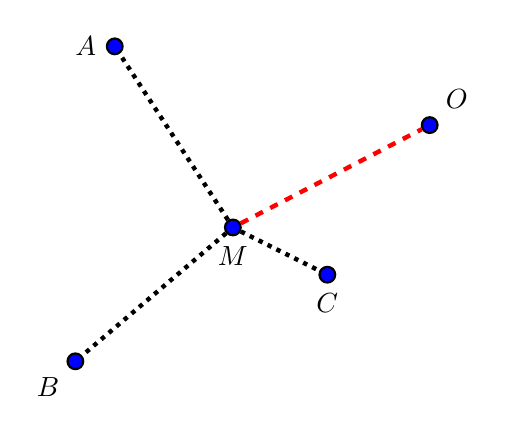
\begin{tikzpicture}[dot/.style={circle, fill=blue, draw=black, thick, inner sep=2pt}, node distance=2cm]
			\node[dot, label=left:{$A$}] (A) at (-1.5, 2.5) {};
			\node[dot, label=below left:{$B$}] (B) at (-2, -1.5) {};
			\node[dot, label=below:{$C$}] (C) at (1.2, -0.4) {};
			\node[dot, label=above right:{$O$}] (O) at (2.5, 1.5) {};
			\node[dot, label=below:{$M$}] (M) at (0, 0.2) {};
			\draw[dotted, ultra thick] (M) -- (B);
			\draw[dotted, ultra thick] (M) -- (C);
			\draw[dotted, ultra thick] (M) -- (A);
			\draw[dashed, red, ultra thick] (M) -- (O);
	\end{tikzpicture}}
	\noindent
	Vật thứ nhất đi từ $M$ đến ba điểm $A$, $B$, $C$ rồi trở về $M$ (có thể được phép trở về $M$ nhiều lần).
	Vật thứ hai đi từ $M$ đến $O$ rồi trở về $M$. Hãy tính theo giây, giá trị nhỏ nhất của tổng thời gian vật thứ nhất đã đi nhiều hơn so với vật thứ hai \textit{(làm tròn kết quả đến hàng phần mười)}.
	\par
	\shortans[0]{50{,}3}
	\loigiai{
		\begin{itemize}
			\item Thời gian vật thứ nhất đi là $t_1=\dfrac{2\cdot\left(MA+MB+MC\right)}{20} = \dfrac{MA+MB+MC}{10}$ giây.
			\item Thời gian vật thứ hai đi là $t_2=\dfrac{2\cdot MO}{20} = \dfrac{MO}{10}$ giây.
		\end{itemize}
		Khi đó, tổng thời gian vật thứ nhất đi nhiều hơn vật thứ hai là \[\Delta t = t_1 - t_2 = \dfrac{MA+MB+MC-MO}{10}.\]
		Ta cần tìm $\min \left(MA+MB+MC-MO\right)$.\\
		Áp dụng bất đẳng thức tam giác ta có
		\begin{itemize}
			\item $MA+MB \geq AB$, dấu đẳng thức xảy ra khi $A$, $M$, $B$ theo thứ tự thẳng hàng.
			\item $\left|MC-MO\right| \leq OC \Leftrightarrow -OC \leq MC-MO \leq OC$, dấu đẳng thức xảy ra khi $M$, $C$, $O$ theo thứ tự thẳng hàng.
		\end{itemize}
		Do đó $MA+MB+MC-MO \geq AB - OC = 2\sqrt{14} - \sqrt{6} \approx 5{,}033$.\\
		Vì đơn vị độ dài trên mỗi trục là $100$ mét nên $\min \Delta t = \dfrac{5{,}033 \cdot 100}{10}=50{,}3$ giây.
	}
\end{ex}
%%%=============================%%%

%%%=============EX_22=============%%%
\begin{ex}%[0D8C2-5]%[TDMT08]%[Nguyễn Thành Hậu]
	\immini[thm]{Cho tập $X=\{1; 2; 3; 4; 5; 6; 7; 8; 9; 10; 11\}$ và $7$ ô hình tròn được bố trí như hình vẽ bên dưới. Với mỗi ô hình tròn ta điền tối đa một số từ tập $X$ và không có hai ô nào được điền cùng một số. Hỏi có bao nhiêu cách chọn ra $7$ số từ tập hợp $X$ để xếp vào $7$ ô hình tròn, sao cho cứ ba ô hình tròn thẳng hàng đều chứa số $5$, tổng của ba ô hình tròn thẳng hàng là bằng nhau?}{	
		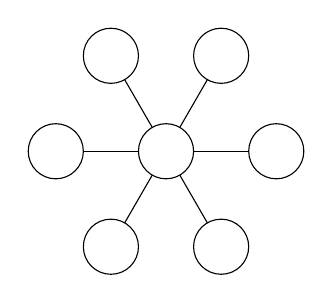
\begin{tikzpicture}[declare function={r=0.5; R=2;}, line cap=round, line join=round, >=stealth, font=\footnotesize, scale=0.7]
			\draw (180:R) coordinate (4) -- (0,0) coordinate (7) -- (0:R) coordinate (1);
			\draw (-120:R) coordinate (5) -- (0,0) coordinate (7) -- (60:R) coordinate (2);	
			\draw (-60:R) coordinate (6) -- (0,0) coordinate (7) -- (120:R) coordinate (3);	
			\foreach \u in {7,1,2,3,4,5,6} {
				\filldraw[fill=white, draw=black] (\u) circle (r);
			}
	\end{tikzpicture}}
	\par
	\shortans[0]{960}
	\loigiai{\immini{Giả sử các số được điền vào các ô hình tròn lần lượt là $a_{1},\ldots,a_{7}$ như hình vẽ.\\
			Theo đề bài $a_{1}+a_{4}+a_{7}=a_{2}+a_{5}+a_{7}=a_{3}+a_{6}+a_{7}\Rightarrow a_{1}+a_{4}=a_{2}+a_{5}=a_{3}+a_{6}$.\\
			Khi đó, $a_{1}+a_{2}+a_{3}+a_{4}+a_{5}+a_{6}=\left(a_{1}+a_{4}\right)+\left(a_{2}+a_{5}\right)+\left(a_{3}+a_{6}\right)$.\\
			Vì ba ô thẳng hàng nào cũng chứa số $5$ nên bắt buộc số $5$ phải nằm ở tâm, tức là $a_{7}=5$. Có $1$ cách xếp số $5$.\\
			Khi đó $a_{i}$ đều khác $5$ với mọi $i=\overline{1,6}$.}{
			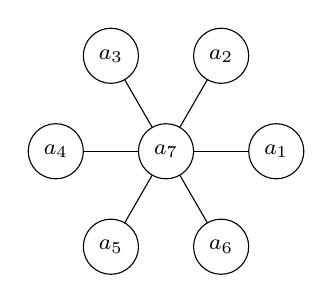
\begin{tikzpicture}[declare function={r=0.5; R=2;}, line cap=round, line join=round, >=stealth, font=\footnotesize, scale=0.7]
				\draw (0,0) coordinate (7) -- (0:R) coordinate (1);
				\draw (0,0) coordinate (7) -- (60:R) coordinate (2);	
				\draw (0,0) coordinate (7) -- (120:R) coordinate (3);	
				\draw (0,0) coordinate (7) -- (180:R) coordinate (4);
				\draw (0,0) coordinate (7) -- (-120:R) coordinate (5);
				\draw (0,0) coordinate (7) -- (-60:R) coordinate (6);
				\foreach \i in {7,1,2,3,4,5,6} {
					\filldraw[fill=white, draw=black] (\i) circle (r);
					\node at (\i) {$a_{\i}$};
				}
		\end{tikzpicture}}
		\noindent
		Sáu số điền vào các ô xung quanh tạo thành $3$ cặp đối xứng có tổng bằng nhau. Ta cần chọn $3$ cặp số phân biệt từ tập $X \setminus \{5\} = \{1; 2; 3; 4; 6; 7; 8; 9; 10; 11\}$ sao cho tổng mỗi cặp đều bằng $S$.\\
		Ta thống kê số lượng các cặp có cùng tổng $S$ được tạo ra từ tập $X \setminus \{5\}$:
		\begin{itemize}
			\item Với $S=9$: có $3$ cặp $(1,8), (2,7), (3,6) \Rightarrow$ Có $\mathrm{C}_3^3=1$ cách chọn ra $3$ cặp.
			\item Với $S=10$: có $4$ cặp $(1,9), (2,8), (3,7), (4,6) \Rightarrow$ Có $\mathrm{C}_4^3=4$ cách chọn ra $3$ cặp.
			\item Với $S=11$: có $4$ cặp $(1,10), (2,9), (3,8), (4,7) \Rightarrow$ Có $\mathrm{C}_4^3=4$ cách chọn.
			\item Với $S=12$: có $4$ cặp $(1,11), (2,10), (3,9), (4,8) \Rightarrow$ Có $\mathrm{C}_4^3=4$ cách chọn.
			\item Với $S=13$: có $4$ cặp $(2,11), (3,10), (4,9), (6,7) \Rightarrow$ Có $\mathrm{C}_4^3=4$ cách chọn.
			\item Với $S=14$: có $3$ cặp $(3,11), (4,10), (6,8) \Rightarrow$ Có $\mathrm{C}_3^3=1$ cách chọn.
			\item Với $S=15$: có $3$ cặp $(4,11), (6,9), (7,8) \Rightarrow$ Có $\mathrm{C}_3^3=1$ cách chọn.
			\item Với $S=17$: có $3$ cặp $(6,11), (7,10), (8,9) \Rightarrow$ Có $\mathrm{C}_3^3=1$ cách chọn.
		\end{itemize}
		\textit{(Các tổng $S$ khác như $7, 8, 16$ chỉ tạo được tối đa $2$ cặp nên không đủ để chọn)}.\\
		Suy ra, số cách chọn ra bộ $3$ cặp thỏa mãn là: 
		\[N_2 = 4 \cdot \mathrm{C}_4^3 + 4 \cdot \mathrm{C}_3^3 = 4 \cdot 4 + 4 \cdot 1 = 20 \text{ (cách)}.\]
		Với mỗi bộ $3$ cặp số được chọn, ta tiến hành xếp chúng vào $6$ vị trí xung quanh tâm:
		\begin{itemize}
			\item Xếp $3$ cặp vào $3$ đường thẳng đi qua tâm: có $3!$ cách.
			\item Trên mỗi đường thẳng, $2$ số của cặp có thể đổi chỗ cho nhau: có $2^3$ cách.
		\end{itemize}
		Suy ra mỗi bộ $3$ cặp số có $3! \cdot 2^3 = 48$ cách xếp.\\
		Vậy có tất cả $1 \cdot 20 \cdot 48 = 960$ cách xếp thỏa mãn yêu cầu bài toán.
	}
\end{ex}
%%%=============================%%%
\Closesolutionfile{ans}
\newpage
\indapan{12}{ans/ansTN-Dung}
\indapan[TF]{2}{ans/ansTN-DungSai}
\indapan[SA]{6}{ans/ansTN-DienKhuyet}
%%%%%%%%%%%%%%
%%nhãn kết thúc đề (để đếm số trang tự động mỗi đề)
\label{B\thedeso}